\documentclass[10pt,a4paper]{article}

\usepackage{polski}
\usepackage[utf8]{inputenc}
\usepackage[polish]{babel}
\usepackage{hhline}
\usepackage{pgfplots}
\usepackage{multicol}
\usepackage{multirow}
%\usepackage{slashbox}
\usepackage{graphicx}
\usepackage{caption}
\usepackage{subcaption}
\usepackage{colortbl}
\usepackage{geometry}
\usepackage{listings}
\usepackage{mathtools}
\DeclarePairedDelimiter\ceil{\lceil}{\rceil}
\DeclarePairedDelimiter\floor{\lfloor}{\rfloor}
\geometry{a4paper, total={170mm,257mm}, left=20mm, top=20mm }
\lstset
{
    language=C++,
    basicstyle=\footnotesize,
    numbers=left,
    stepnumber=1,
    showstringspaces=false,
    tabsize=1,
    breaklines=true,
    breakatwhitespace=false,
}
\author{Sebastian Maciejewski 132275 i Jan Techner 132332\\
grupa I1, zajęcia we wtorki o 15:10, tygodnie nieparzyste,\\
email: maciejewski.torun@gmail.com}
\title{Badanie wpływu organizacji dostępu do pamięci globalnej na efektywność
przetwarzania - Nvidia CUDA}
\date{11 czerwca 2019}
\setlength{\parindent}{0pt}
\newcommand{\forceindent}{\leavevmode{\parindent=3em\indent}}
\begin{document}
\maketitle
\section{Wstęp}
Sprawozdanie dotyczy zadania w wariancie 5. - badanie wpływu organizacji dostępu do
pamięci globalnej (dostęp łączony i dostęp niełączony) na efektywność przetwarzania.\\
Warianty kodu:\\
- grid wieloblokowy, obliczenia przy wykorzystaniu pamięci globalnej,\\
- grid wieloblokowy, obliczenia przy wykorzystaniu pamięci współdzielonej bloku wątków.\\
Każdy z tych wariantów był wykorzystywany w dwóch wersjach - z łączonym oraz niełączonym
dostępem do pamięci. Zastosowaliśmy dwa rozmiary bloków - 8x8 i 16x16, a pomiary pobraliśmy
dla instancji o różnych wielkościach (128x128, 256x256, 512x512, 864x864, 1024x1024).

Wszystkie pomiary zostały wykonane na komputerach laboratoryjnych w sali 2.7.6. na karcie
Nvidia GTX 260.

\subsection{Specyfikacja sprzętu i wykorzystanego oprogramowania}
\begin{itemize}
	\item karta graficzna Nvidia GTX 260
	      \begin{itemize}
	      	\item compute capability - 1.3
	      	\item liczba multiprocesorów - 27
	      	\item maksymalna liczba bloków na jeden multiprocesor - 8
	      	\item maksymalna liczba wątków w bloku - 512
	      	\item warp size - 32
	      	\item half-warp size - 16
	      \end{itemize}
	\item Visual Studio 2013
	\item Nvidia Visual Profiler
\end{itemize}

\section{Analiza przygotowania eksperymentu}
\subsection{Kod wykorzystywany przy pomiarach}
\subsubsection*{Obliczenia z wykorzystaniem pamięci globalnej}
W pierwszym wariancie kodu do obliczeń wykorzystujemy pamięć globalną - fragmenty
pamięci zarezerwowane na każdą z 3 macierzy za pomocą cudaMalloc. Każdy z wątków
oblicza jeden element wynikowy dodając wartości w swoim lokalnym rejestrze (C\_local),
po czym zapisuje wynik takiego przetwarzania do tablicy w pamięci globalnej.

\subsubsection*{Obliczenia z wykorzystaniem pamięci współdzielonej bloku wątków}
W drugim wariancie wykorzystujemy współdzieloną pamięć bloku wątków. Pewien obszar
pamięci został zaalokowany na współdzielony obszar pamięci bloku wątków za pomocą
\_\_shared\_\_. Dwa takie obszary, o rozmiarze 8x8 lub 16x16 (w zależności od pomiaru)
odpowiadają za przechowywanie fragmentów mnożonej macierzy. Dla każdego bloku wątków
dane są pobierane do jego pamięci współdzielonej, następnie każdy z wątków wylicza
na ich podstawie swój wynik. \\
Taka organizacja przetwarzania mogłaby prowadzić do problemów z np. nadpisywaniem danych,
więc konieczna jest synchronizacja - aby 'poczekać' na zakończenie przetwarzania przez wszystkie wątki, wywoływana
jest funkcja \_\_syncthreads. Po zakończeniu przetwarzania, wynik jest zapisywany w
pamięci globalnej.


\subsubsection{Rodzaje dostępu do pamięci}
Dostęp do pamięci w kartach graficznych Nvidia odbywa się za pomocą transkacji o rozmiarach
32, 64 lub 128 bitów. W karcie na której przeprowadzany był eksperyment (CC 1.3) takie dostępy
są realizowane dla tzw. half-wrapów - 16 wątkowych grup. \\
Różnica między dostępem łączonym a niełączonym sprowadza się do tego, że
dostępem łączonym nazywamy dostęp do pamięci tych wątków half-wrapu, które
sąsiadują ze sobą w pamięci. Dostęp w przeciwnym wypadku (wątki nie siąsiadują ze sobą
w pamięci) nazywany jest dostępem niełączonym.

\newpage

\subsection{Istotne fragmenty kodu}
\subsubsection*{Wariant G\_L - dostęp łączony, pamięć globalna}
\begin{lstlisting}
	template <int BLOCK_SIZE> __global__ void matrixMulCUDA(float *C, float *A,
	float *B, int wA,
	int wB) {
	// Block index
	int bx = blockIdx.x;
	int by = blockIdx.y;

	// Thread index
	int tx = threadIdx.x;
	int ty = threadIdx.y;

	int row = by * blockDim.y + ty;
	int col = bx * blockDim.x + tx;
	float C_local = 0;

	for (int k = 0; k < wA; k++) {
		C_local += A[row*wA + k] * B[k *wA + col];
	}

	C[row*wA + col] = C_local;
}
\end{lstlisting}

\subsubsection*{Wariant G\_NL - Dostęp niełączony, pamięć globalna}
\begin{lstlisting}
	template <int BLOCK_SIZE> __global__ void matrixMulCUDA(float *C, float *A,
	float *B, int wA,
	int wB) {
	// Block index
	int bx = blockIdx.x;
	int by = blockIdx.y;

	// Thread index
	int tx = threadIdx.x;
	int ty = threadIdx.y;

	int col= by * blockDim.y + ty;
	int row = bx * blockDim.x + tx;
	float C_local = 0;

	for (int k = 0; k < wA; k++) {
		C_local += A[row*wA + k] * B[k *wA + col];
	}

	C[row*wA + col] = C_local;
}
\end{lstlisting}

\subsubsection*{Wariant S\_L - dostęp łączony, pamięć współdzielona bloku wątków}
\begin{lstlisting}
	template <int BLOCK_SIZE> __global__ void matrixMulCUDA(float *C, float *A,
	float *B, int wA,
	int wB) {
	// Block index
	int bx = blockIdx.x;
	int by = blockIdx.y;

	// Thread index
	int tx = threadIdx.x;
	int ty = threadIdx.y;

	int row = by * blockDim.y + ty;
	int col = bx * blockDim.x + tx;
	float C_local = 0;

	__shared__ float matAhelp[BLOCK_SIZE][BLOCK_SIZE];
	__shared__ float matBhelp[BLOCK_SIZE][BLOCK_SIZE];
	for (int m = 0; m < wA / BLOCK_SIZE; ++m) {
		matAhelp[tx][ty] = A[row * wA + m*BLOCK_SIZE + tx];
		matBhelp[tx][ty] = B[(m*BLOCK_SIZE + ty)*wA + col];
		__syncthreads();
		for (int k = 0; k < BLOCK_SIZE; ++k)
			C_local += matAhelp[tx][k] * matBhelp[k][ty];
		__syncthreads();
	}

	C[row*wA + col] = C_local;
}
\end{lstlisting}

\subsubsection*{Wariant S\_NL - dostęp niełączony, pamięć współdzielona bloku wątków}
\begin{lstlisting}
	template <int BLOCK_SIZE> __global__ void matrixMulCUDA(float *C, float *A,
	float *B, int wA,
	int wB) {
	// Block index
	int bx = blockIdx.x;
	int by = blockIdx.y;

	// Thread index
	int tx = threadIdx.x;
	int ty = threadIdx.y;

	int col = by * blockDim.y + ty;
	int row = bx * blockDim.x + tx;
	float C_local = 0;

	__shared__ float matAhelp[BLOCK_SIZE][BLOCK_SIZE];
	__shared__ float matBhelp[BLOCK_SIZE][BLOCK_SIZE];
	for (int m = 0; m < wA / BLOCK_SIZE; ++m) {
		matAhelp[tx][ty] = A[row * wA + m*BLOCK_SIZE + tx];
		matBhelp[tx][ty] = B[(m*BLOCK_SIZE + ty)*wA + col];
		__syncthreads();
		for (int k = 0; k < BLOCK_SIZE; ++k)
			C_local += matAhelp[tx][k] * matBhelp[k][ty];
		__syncthreads();
	}

	C[row*wA + col] = C_local;
}
\end{lstlisting}

\subsubsection*{Wizualizacja przetwarzania}
Na poniższych grafikach widać różnicę w procesie obliczania macierzy z wykorzystaniem
pamięci globalnej i pamięci współdzielonej wątków.\\

\begin{figure}[h]
	\centering
	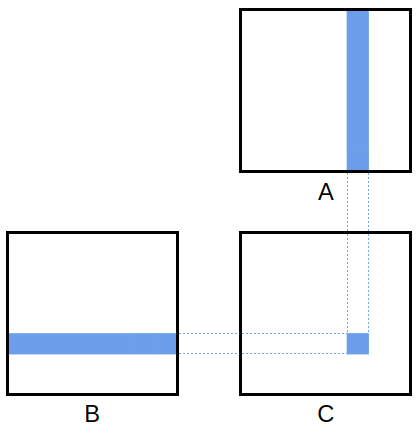
\includegraphics[width=0.5\textwidth]{1.png}
	\caption{Wykorzystanie pamięci globalnej}
\end{figure}

\begin{figure}[h]
	\centering
	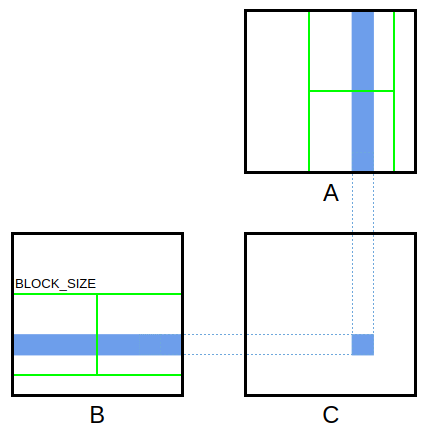
\includegraphics[width=0.5\textwidth]{2.png}
	\caption{Wykorzystanie pamięci podręcznej, dostęp niełączony}
\end{figure}

W przypadku pamięci globalnej każdy wątek odczytuje jeden wiersz macierzy A i jedną
kolumnę macierzy B, a następnie oblicza odpowiadający element macierzy C. Wszystkie
dane odczytywane są bezpośrednio z pamięci globalnej, co powoduje bardzo dużą liczbę odwołań
do pamięci globalnej.\\
W drugim przypadku, dla pamięci współdzielonej bloku wątków, każdy blok oblicza macierz
będącą częścią macierzy wynikowej C o rozmiarze równym rozmiarowi bloku. Każdy wątek
jest wówczas odpowiedzialny za obliczenie jednego elementu takiego wycinka macierzy.
W taki sposób znacząco ograniczamy ilość dostępów do pamięci globalnej, ponieważ macierze
A i B są odczytywane tylko $\frac{n}{BLOCK\_SIZE}$ razy, gdzie $n$ to wielkość instancji a
$BLOCK\_SIZE$ to wielokść bloku.

\section{Analiza wyników eksperymentu pomiarowego}
\subsection{Miary efektywności}
\subsubsection*{Prędkość obliczeń}
\begin{equation}
	\frac{ZL}{t} = \frac{2 * n^3}{t}
\end{equation}
gdzie $ZL$ to złożoność obliczeniowa, $t$ to czas, a $n$ to rozmiar instancji.

\subsubsection*{Przyspieszenie w stosunku do IKJ}
\begin{equation}
	\frac{t_{IKJ}}{CPR}
\end{equation}
gdzie $t_{IKJ}$ to czas przetwarzania IKJ a $CPR$ to czas przetwarzania równoległego.

\subsubsection*{Przyspieszenie w funkcji wielkości instancji}
\begin{equation}
	\frac{CPI}{CP 128}
\end{equation}
gdzie $CPI$ to czas przetwarzania dla instancji a $CPI 128$ to czas przetwarzania dla
instancji o rozmiarze 128, będący naszym punktem odniesienia - obliczamy przyspieszenie
w stosunku do przetwarzania instancji o rozmiarze 128.

\subsubsection*{Miara stopnia łączenia dostępów do pamięci}
Jest to miara obliczana w następujący sposób: dla każdebo bloku pobierane
będą dwie macierze ($n^2$), dodajemy do tego $n^2$ zapisów do pamięci globalnej
i dzielimy przez sumę transkacji między pamięcią a multiprocesorem (odczytane
z wyników z programu Visual Profiler).\\

\subsubsection*{Zajętość procesora}
Wyliczana za pomocą kalkulatora zajętości SM miara - dla bloków o rozmiarze
8x8 osiąga $50\%$, zaś dla bloków o rozmiarze 16x16 osiąga $100\%$, czego można
się było spodziewać. Pokazuje to, że pełnię możliwości tej karty wykorzystujemy
wtedy, gdy bloki mają rozmiar 16x16.

\subsubsection*{CGMA - stosunek operacji do dostępów do pamięci}
Jest to miara instensywności obliczeń. Zakładamy, że do obliczenia jednego elementu
wynikowego potrzebujemy n danych z wiersza macierzy, n danych z kolumny macierzy
oraz 1 operację zapisu do pamięci globalnej.\\
Warto zauważyć, że dla współdzielonej pamięci bloku wątków CGMA będzie bliski 1,
ponieważ pomijamy operacje pobierania danych z pamięci globalnej do lokalnej.

gdzie $n$ to wielkość instancji.

\subsubsection*{GLD\_EFFICIENCY}
Jest to miara efektywności pobierania danych z pamięci globalnej obliczana w sposób
następujący:
\begin{equation}
	\frac{gld\_reques}{gld\_total / (2*SM)}
\end{equation}
gdzie $SM$ to liczba multiprocesorów.

\subsubsection*{GST\_EFFICIENCY}
Jest to miara efektywności zapisu danych w pamięci globalnej.
Oblicza się ją analogicznie
do GLD\_EFFICIENCY.
\begin{equation}
	\frac{gst\_reques}{(gst\_32 + gst\_64 + gst\_128) / (2*SM)}
\end{equation}
gdzie $SM$ to liczba multiprocesorów.

\subsection{Wyniki pomiarów}

\begin{table}
											
											
\end{table}

\begin{center}
	\begin{tabular}{ |c|c|c|c|c|c|c|c|c|c|c|c| }
		\hline
		V                       & BS                  & INST & T[ms]  & GFLOPS & vs IKJ & $\Delta A$ & CMGA   & JOIN     & \%    & GLD\_E   & GST\_E  \\ \hline
		\multirow{10}{*}{G\_L}  & \multirow{5}{*}{8}  & 128  & 0,17   & 25,32  & 12,07  & 1,00       & 0,0039 & 733,88   & 50\%  & 5184     & 141208  \\ \cline{3-12}
		                        &                     & 256  & 1,10   & 30,63  & 2,74   & 6,61       & 0,0019 & 1512,50  & 50\%  & 10368    & 10904   \\ \cline{3-12}
		                        &                     & 512  & 10,20  & 26,33  & 2,65   & 61,55      & 0,0010 & 3045,11  & 50\%  & 20736    & 591     \\ \cline{3-12}
		                        &                     & 864  & 58,03  & 22,23  & 2,43   & 350,32     & 0,0006 & 5162,90  & 50\%  & 34992    & 59      \\ \cline{3-12}
		                        &                     & 1024 & 87,08  & 24,66  & 5,87   & 525,70     & 0,0005 & 6121,00  & 50\%  & 41472    & 35      \\ \cline{2-12}
		                        & \multirow{5}{*}{16} & 128  & 0,12   & 33,95  & 16,19  & 1,00       & 0,0039 & 245,81   & 100\% & 1728     & 282894  \\ \cline{3-12}
		                        &                     & 256  & 1,03   & 32,58  & 2,91   & 8,34       & 0,0019 & 552,75   & 100\% & 3456     & 17551   \\ \cline{3-12}
		                        &                     & 512  & 7,80   & 34,41  & 3,46   & 63,14      & 0,0010 & 1136,81  & 100\% & 6912     & 1141    \\ \cline{3-12}
		                        &                     & 864  & 39,38  & 32,75  & 3,58   & 318,82     & 0,0006 & 1930,81  & 100\% & 11664    & 133     \\ \cline{3-12}
		                        &                     & 1024 & 71,83  & 29,90  & 7,11   & 581,49     & 0,0005 & 2286,30  & 100\% & 13824    & 63      \\ \cline{1-12}
		\multirow{10}{*}{G\_NL} & \multirow{5}{*}{8}  & 128  & 0,41   & 10,11  & 4,82   & 1,00       & 0,0039 & 242,44   & 50\%  & 3888     & 77004   \\ \cline{3-12}
		                        &                     & 256  & 3,47   & 9,66   & 0,86   & 8,37       & 0,0019 & 501,87   & 50\%  & 7776     & 4603    \\ \cline{3-12}
		                        &                     & 512  & 44,66  & 6,01   & 0,60   & 107,67     & 0,0010 & 1012,71  & 50\%  & 15552    & 181     \\ \cline{3-12}
		                        &                     & 864  & 204,65 & 6,30   & 0,69   & 493,37     & 0,0006 & 1718,62  & 50\%  & 26244    & 23      \\ \cline{3-12}
		                        &                     & 1024 & 504,72 & 4,25   & 1,01   & 1216,81    & 0,0005 & 2037,98  & 50\%  & 31104    & 8       \\ \cline{2-12}
		                        & \multirow{5}{*}{16} & 128  & 0,81   & 5,15   & 2,45   & 1,00       & 0,0039 & 29,13    & 100\% & 3672     & 41510   \\ \cline{3-12}
		                        &                     & 256  & 6,52   & 5,15   & 0,46   & 8,00       & 0,0019 & 65,27    & 100\% & 7344     & 2595    \\ \cline{3-12}
		                        &                     & 512  & 75,20  & 3,57   & 0,36   & 92,30      & 0,0010 & 134,00   & 100\% & 14688    & 112     \\ \cline{3-12}
		                        &                     & 864  & 388,92 & 3,32   & 0,36   & 477,38     & 0,0006 & 227,41   & 100\% & 24786    & 13      \\ \cline{3-12}
		                        &                     & 1024 & 990,65 & 2,17   & 0,52   & 1215,98    & 0,0005 & 269,23   & 100\% & 29376    & 4       \\ \cline{1-12}
		\multirow{10}{*}{S\_L}  & \multirow{5}{*}{8}  & 128  & 0,13   & 33,10  & 15,78  & 1,00       & 1      & 3879,09  & 50\%  & 864      & 1112210 \\ \cline{3-12}
		                        &                     & 256  & 0,86   & 38,81  & 3,47   & 6,82       & 1      & 8493,26  & 50\%  & 1728     & 82978   \\ \cline{3-12}
		                        &                     & 512  & 6,85   & 39,20  & 3,94   & 54,03      & 1      & 17661,66 & 50\%  & 3456     & 5254    \\ \cline{3-12}
		                        &                     & 864  & 54,47  & 23,68  & 2,59   & 429,82     & 1      & 25701,09 & 50\%  & 6912     & 330     \\ \cline{3-12}
		                        &                     & 1024 & 32,73  & 65,60  & 15,61  & 258,29     & 1      & 42639,10 & 50\%  & 5832     & 652     \\ \cline{2-12}
		                        & \multirow{5}{*}{16} & 128  & 0,24   & 17,17  & 8,19   & 1,00       & 1      & 2352,76  & 100\% & 0        & 2155375 \\ \cline{3-12}
		                        &                     & 256  & 1,61   & 20,78  & 1,86   & 6,61       & 1      & 6582,70  & 100\% & 0        & 170279  \\ \cline{3-12}
		                        &                     & 512  & 12,32  & 21,79  & 2,19   & 50,45      & 1      & 15496,47 & 100\% & 0        & 11433   \\ \cline{3-12}
		                        &                     & 864  & 59,10  & 21,83  & 2,39   & 241,97     & 1      & 27996,80 & 100\% & 0        & 1426    \\ \cline{3-12}
		                        &                     & 1024 & 98,48  & 21,81  & 5,19   & 403,22     & 1      & 33641,27 & 100\% & 0        & 724     \\ \cline{1-12}
		\multirow{10}{*}{S\_NL} & \multirow{5}{*}{8}  & 128  & 0,13   & 31,95  & 15,24  & 1,00       & 1      & 1429,14  & 50\%  & 540      & 1726347 \\ \cline{3-12}
		                        &                     & 256  & 0,87   & 38,68  & 3,46   & 6,61       & 1      & 3247,42  & 50\%  & 1080     & 132073  \\ \cline{3-12}
		                        &                     & 512  & 6,86   & 39,14  & 3,94   & 52,25      & 1      & 6899,09  & 50\%  & 2160     & 8390    \\ \cline{3-12}
		                        &                     & 864  & 32,77  & 39,36  & 4,30   & 249,63     & 1      & 11969,10 & 50\%  & 3645     & 1041    \\ \cline{3-12}
		                        &                     & 1024 & 60,00  & 35,79  & 8,52   & 457,02     & 1      & 14265,87 & 50\%  & 4320     & 487     \\ \cline{2-12}
		                        & \multirow{5}{*}{16} & 128  & 0,25   & 16,64  & 7,93   & 1,00       & 1      & 297,64   & 100\% & 229,5    & 2118706 \\ \cline{3-12}
		                        &                     & 256  & 1,65   & 20,39  & 1,82   & 6,53       & 1      & 810,56   & 100\% & 459      & 164427  \\ \cline{3-12}
		                        &                     & 512  & 12,36  & 21,72  & 2,18   & 49,04      & 1      & 1871,40  & 100\% & 918      & 10961   \\ \cline{3-12}
		                        &                     & 864  & 59,12  & 21,82  & 2,39   & 234,54     & 1      & 3348,45  & 100\% & 1549,125 & 1358    \\ \cline{3-12}
		                        &                     & 1024 & 98,54  & 21,79  & 5,19   & 390,94     & 1      & 4014,01  & 100\% & 1836     & 688     \\ \cline{1-12}
	\end{tabular}
	\captionof{table}{Miary efektywności dla 6 pętli, przetwarzanie równolegle}
\end{center}

Nazwy kolumn:
\begin{itemize}
	\item V - wersja kodu 
	\item BS - rozmiar bloku 
	\item INST - rozmiar instancji (długość boku macierzy)
	\item T[ms] - czas przetwarzania w ms 
	\item GFLOPS - prędkość przetwarzania
	\item vs IKJ - przyspieszenie w stosunku do IJK 
	\item $\Delta A$ - zmiana przyspieszenia w funkcji wielkości instancji
	\item JOIN - miara stopnia łączenia dostępów do pamięci globalnej
	\item \% - zajętość multiprocesora
	\item GLD\_E - gld\_efficiency 
	\item GST\_E - gst\_efficiency
\end{itemize}


\section{Wnioski}
Po przeanalizowaniu wyników


\end{document}